
\vspace{1cm}{\bf ECal performance [Sho]}

The ECal preamplifiers shape the APD signal into a CR-RC pulse of rise time $\approx 14$~ns: this is sampled every 4~ns and stored in a pipeline on the FADC readout board. On receiving a trigger, the FADC searches for rising threshold crossings in the pipeline and integrates pulses by summing 5 samples before and 30 samples after each threshold crossing. The noise and pedestal of the readout chain are calibrated by running the ECal readout in a mode where the preamplifier output is sampled every 4~ns in a time window of 100 samples: by looking at a part of the window before the hit, we calibrate the readout channel.

Of 442 crystals/channels, 39 were disabled or disconnected and were not read out by the DAQ. 
13 of these were not read out because of a shortage of FADC readout boards.
The remainder either had no HV bias on the APD, or were disabled in the FADC software due to noise.
In the data, we identified two types of abnormal channels. 
One FADC was not sending trigger signals correctly, resulting in low efficiency. This affected the 13 channels read out by that FADC.
5 channels were diagnosed as noisy because they had a high incidence of hits out of coincidence with the trigger.
A large number of channels were originally misidentified as noisy because they had much higher hit occupancy than neighboring channels.
Gain calibration (described in the next section) shows that these channels have high gain (and thus lower energy threshold) but are otherwise normal.
The abnormal channels were ignored in analysis in order to simplify comparison with Monte Carlo. This leaves 385 useful channels---87\% of the ECal.

We found that one quadrant of the ECal had been miswired in such a way as to flip the horizontal coordinate---the column of crystals nearest the center was connected to the readout channels for the rightmost column, and vice versa.
\begin{figure}[ht]
	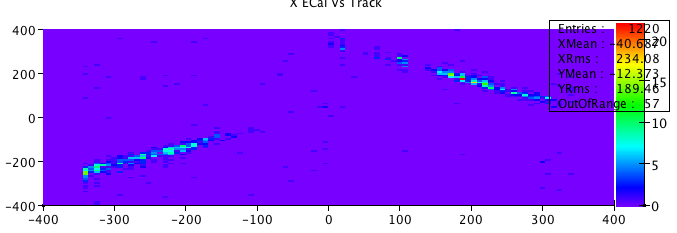
\includegraphics[width=\textwidth]{test2012/ecalperformance/x_match_flip}
	%\includegraphics[width=0.4\textwidth]{test2012/ecalperformance/crystal_edges_flip}
	\caption{\small{ECal hit position from track extrapolation vs. ECal hit position from ECal (for top half of ECal only). Shows that $x>0$ quadrant is flipped.}}
	\label{fig:x_flip}
\end{figure}

\begin{figure}[ht]
	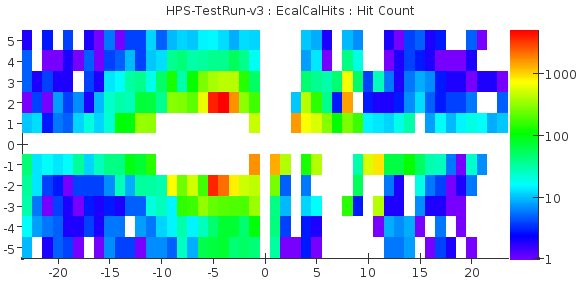
\includegraphics[width=0.5\textwidth]{test2012/ecalperformance/hitrates}
	\caption{\small{Hit rates (above an energy threshold, to cut out effect of gain variations) vary smoothly with position.}}
	\label{fig:hitrates}
\end{figure}
For ECal analysis, cluster reconstruction was done using the algorithm described in \cite{HPS_PROP}: build clusters around seed hits (hits above a ``seed'' energy threshold and with greater energy than any neighboring hits), and add all neighboring hits above an ``add'' energy threshold.

\vspace{1cm}{\bf ECal Calibration [Sho]}

We calibrate gain of the individual ECal channels using the SVT measurement of track momentum. 
The ratio of cluster energy to track momentum is calculated both for Monte Carlo simulation and test run data at each point in the ECal, and we find the value of gain for each channel that brings the two into agreement.
We use a formula to compute the ``weighted E/p'' for a crystal, representing the average E/p for clusters that include the crystal: $\frac{\sum_j w_{j,i}}{\sum_j\frac{P_j}{E_j}w_{j,i}}$.
We disable all SVT and ECal channels in the simulation that were inoperable or noisy in the test run, so any efficiency or bias effects that affect the real data should be reflected in the simulation as well.

The calibrated gains are corrected by the ratio between the weighted E/p values from Monte Carlo and real data.
The E/p in Monte Carlo data is also affected by the gain because the trigger thresholds change, so both Monte Carlo and data reconstruction are rerun with each iteration of gain calibration.
It takes up to 4 iterations for the gains to stabilize; the final values are shown in Figure \ref{fig:gains}.
\begin{figure}[ht]
	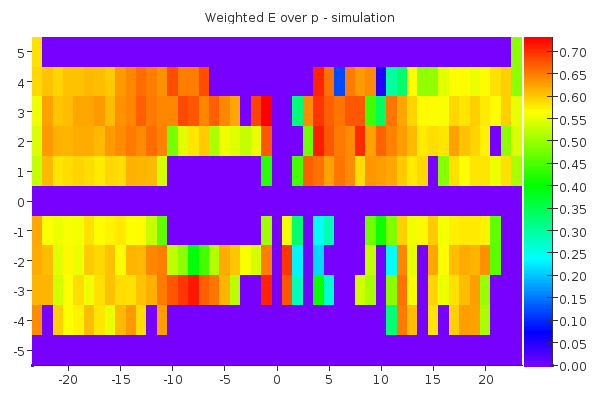
\includegraphics[width=0.45\textwidth]{test2012/ecalperformance/ecalgainplots_corr_sim}
	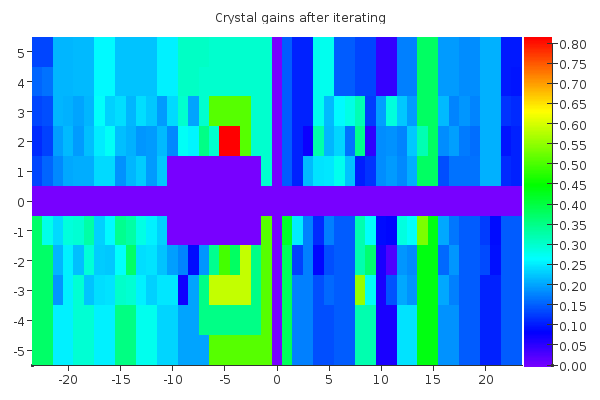
\includegraphics[width=0.45\textwidth]{test2012/ecalperformance/gains}
	\caption{\small{Weighted E/p from Monte Carlo simulation (left), calibrated values of gain in units of MeV per ADC count (right).}}
	\label{fig:gains}
\end{figure}
These gains can then be used to convert from ADC counts in a channel to energy deposited into that ECal crystal.
The other information needed to find the energy of an incident particle is the sampling fraction---the ratio of energy read out from crystals to energy of an incident particle.
The conventional sampling fraction---the fraction of incident energy that is deposited in crystals---is approximately 0.9 for our ECal, and less at edges.
For our readout, there is additional energy lost because crystals under the readout threshold are not read out.
The weighted E/p used in calibration (see Figure \ref{fig:gains}) is an approximate measurement of sampling fraction, but the sampling fraction is energy-dependent because of the effect of readout threshold.

\vspace{1cm}{\bf Trigger performance [Sho/Ben]}

%\begin{figure}[ht]
%	\includegraphics[width=\textwidth]{test2012/ecalperformance/trigtimes}
%	\caption{\small{}}
%	\label{fig:trigtimes}
%\end{figure}

As described in Section \ref{sec:testrun_trigger}, the trigger and DAQ integrate pulses differently to measure hit energy. The trigger integrates using a time-over-threshold window, and the DAQ readout integrates using a constant window (5 samples before and 30 samples after a threshold crossing). 
For every event, the trigger reports as a bitmask the trigger decision (top trigger, bottom trigger, or both) and the time the trigger fires.

We study trigger performance by simulating the trigger for each event and comparing to how events were actually triggered.
First, we convert from readout hits (constant integration window) to trigger hits (time-over-threshold integration). 
This is done by converting from the readout hit to pulse amplitude, then applying the time-over-threshold algorithm to the simulated ECal pulse shape. 
We then simulate the CTP clustering algorithm and the trigger decision (described in Section \ref{sec:testrun_trigger}), and compare the trigger decision and trigger time reported by the simulation to what was reported by the real trigger.

To eliminate trigger bias in checking the trigger decision, we use a tag and probe method: to check trigger performance in one half of the ECal, we tag events where there was a trigger in the other half, and exactly one probe cluster in the ECal half under test. 
We then measure trigger efficiency (proportion of tagged events where there was a trigger) as a function of ADC counts and energy of the probe cluster.
These turn-on curves are shown for the top half of the ECal in Figure \ref{fig:turnon}. 
The trigger threshold is seen to be 1280 ADC counts as expected. The threshold is not perfectly sharp in this analysis because of uncertainties in the conversion from constant-window to time-over-threshold integrals but based on comparisons with Monte Carlo simulation we believe the trigger worked exactly as specified. 
The trigger threshold in terms of cluster energy is very uneven for two reasons; gain variations between different ECal crystals lead to threshold variations and the nonlinearity of the time-over-threshold integral means that the effective threshold is higher for clusters that span multiple crystals.
\begin{figure}[ht]
	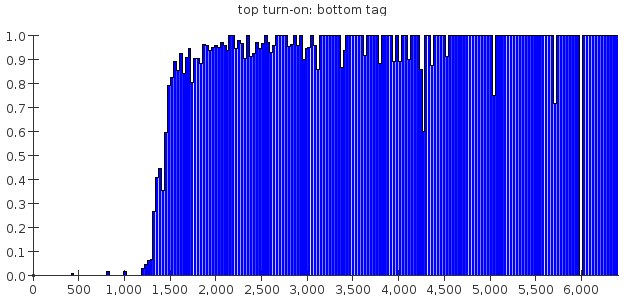
\includegraphics[width=0.4\textwidth]{test2012/ecalperformance/top_turnon_adc}
	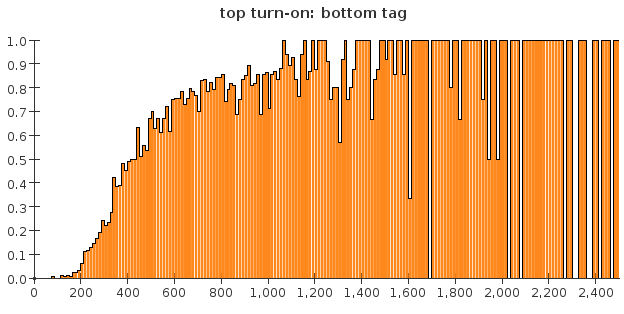
\includegraphics[width=0.4\textwidth]{test2012/ecalperformance/top_turnon_e}
	\caption{\small{Trigger turn-on as a function of probe cluster ADC counts (left) and probe cluster energy in MeV (right). Both plots are for the top half of the ECal; bottom is similar. 
	Energy is not corrected for sampling fraction.}}
	\label{fig:turnon}
\end{figure}
Overall the trigger appears to have functioned exactly as intended. Changes planned for the next run (constant integration window and per-crystal gain calibration constants for the trigger) will solve both of the issues that led to threshold variations in the test run.

{\color{red}
What were the rates, lessons learned?

Plots: rates vs time {\it Ben/Sho/Pelle}}


